
\documentclass[aspectratio=169]{beamer}

% ─── Theme & Colors ───────────────────────────────────────────────────────────
\usetheme{Madrid}
\usecolortheme{rose}
\usepackage{beamerthemeshadow}
\usepackage{graphicx}
\usepackage{booktabs}
\usepackage{tabularx}
\usepackage{multicol}
\usepackage{tikz}
\usepackage{fontenc}
\usepackage{hyperref}

\setbeamertemplate{navigation symbols}{}
\setbeamertemplate{footline}{
  \leavevmode%
  \hbox{%
    \begin{beamercolorbox}[wd=.333333\paperwidth,ht=2.5ex,dp=1ex,center]{author in head/foot}%
      \usebeamerfont{author in head/foot}\insertshortauthor
    \end{beamercolorbox}%
    \begin{beamercolorbox}[wd=.333333\paperwidth,ht=2.5ex,dp=1ex,center]{title in head/foot}%
      \usebeamerfont{title in head/foot}\insertshorttitle
    \end{beamercolorbox}%
    \begin{beamercolorbox}[wd=.333333\paperwidth,ht=2.5ex,dp=1ex,right]{date in head/foot}%
      \insertframenumber{} / \inserttotalframenumber\hspace*{2ex}
    \end{beamercolorbox}}%
  \vskip0pt%
}

\definecolor{nirmablue}{RGB}{0,51,102}
\setbeamercolor{title}{fg=nirmablue}
\setbeamercolor{frametitle}{fg=nirmablue}
\setbeamercolor{block title}{bg=nirmablue,fg=white}
\setbeamercolor{block body}{bg=nirmablue!10}

\markboth{Pravin Kanotara, 22BCE139}{http://www.nirmauni.ac.in}

\title[ChatServe]{Framework for WhatsApp-Based Small Business Automation}
\subtitle{ChatServe -- B.Tech 8th Semester Research Project}
\author[Pravin Kanotara]{Pravin Kanotara (22BCE139)\\ \textit{Guided By: Prof Monika Shah}\\ \small Department of Computer Science \& Engineering}
\institute[Nirma University]{Institute of Technology, Nirma University}
\date{April 2026}

\begin{document}

%==========================================================
% SLIDE 1: Title Slide
%==========================================================
\logo{
\includegraphics[scale=0.15]{Logo.jpg}}
{
\setbeamertemplate{footline}{}
\begin{frame}
\titlepage
\end{frame}
}
\logo{}

%==========================================================
% SLIDE 2: Outline
%==========================================================
\begin{frame}{Outline}
\tableofcontents[hideallsubsections]
\end{frame}

%==========================================================
% SECTION: Introduction & Background
%==========================================================
\section{Introduction \& Background}
\begin{frame}[shrink=5]{Introduction \& Background}

\begin{columns}[T]
\begin{column}{0.55\textwidth}
\begin{itemize}
  \item India has \textbf{6.5 crore+ MSMEs} contributing 30.1\% of GDP
  \item \textbf{500+ million} WhatsApp users in India
  \item Small businesses rely on WhatsApp for customer communication
  \item Manual order handling leads to \textbf{delays, errors, missed messages}
  \item Existing tools are either \textbf{too basic} or \textbf{too expensive}
\end{itemize}
\end{column}
\begin{column}{0.42\textwidth}
\begin{block}{The Gap}
WhatsApp Business App $\rightarrow$ No automation\\[3pt]
WhatsApp Business API $\rightarrow$ Too costly \& complex
\end{block}
\vspace{0.3cm}
\small
\begin{tabular}{lcc}
\toprule
\textbf{Channel} & \textbf{Open} & \textbf{Response} \\
\midrule
WhatsApp & 98\% & 45\% \\
Email & 22\% & 6\% \\
SMS & 95\% & 12\% \\
\bottomrule
\end{tabular}
\end{column}
\end{columns}

\end{frame}

%==========================================================
% SECTION: Problem Statement
%==========================================================
\section{Problem Statement}
\begin{frame}[shrink=5]{Problem Statement}

\begin{block}{Core Problem}
Small businesses using WhatsApp face operational inefficiencies due to the absence of affordable, easy-to-use automation tools tailored to their needs.
\end{block}

\vspace{0.3cm}
\begin{columns}[T]
\begin{column}{0.48\textwidth}
\textbf{Challenges Faced:}
\begin{itemize}
  \item Orders managed manually via chat
  \item No centralized order/booking tracking
  \item High message volume $\rightarrow$ missed orders
  \item No structured workflow or analytics
\end{itemize}
\end{column}
\begin{column}{0.48\textwidth}
\textbf{Market Reality:}
\begin{itemize}
  \item 92\% micro businesses use free WA app
  \item Only 2\% micro businesses use WA API
  \item API platforms cost \textrm{₹}1,500--2,500+/month
  \item Complex setup requires technical expertise
\end{itemize}
\end{column}
\end{columns}

\end{frame}

%==========================================================
% SECTION: Objectives
%==========================================================
\section{Objectives}
\begin{frame}{Project Objectives}

\begin{enumerate}
  \item \textbf{Conversational Onboarding} -- Create a zero-technical-knowledge registration experience entirely via WhatsApp
  \item \textbf{Automated Chatbot} -- Implement WhatsApp-based chatbot for order/booking handling
  \item \textbf{Intuitive Dashboard} -- Provide a simple web interface for catalog and order management
  \item \textbf{Multi-Tenant SaaS} -- Build a scalable architecture serving multiple businesses simultaneously
  \item \textbf{Affordable \& Accessible} -- Keep the system cost-effective and easy to deploy for MSMEs
\end{enumerate}

\begin{block}{Core Research Question}
\textit{How can a small business owner access automated WhatsApp-based order and booking management without technical knowledge, cost burden, or complex setup?}
\end{block}

\end{frame}

%==========================================================
% SECTION: Literature Review
%==========================================================
\section{Literature Review \& Gap Analysis}
\begin{frame}[shrink=10]{Existing Platforms -- Comparative Analysis}

\scriptsize
\renewcommand{\arraystretch}{1.1}
\begin{tabularx}{\textwidth}{|l|X|X|X|X|X|}
\hline
\textbf{Feature} & \textbf{WA Business} & \textbf{Interakt} & \textbf{AiSensy} & \textbf{WATI} & \textbf{Infobip} \\
\hline
Automation & Basic replies & Workflow & Campaign & Chatbot & Advanced \\
\hline
Bot & None & Basic & Rule-based & No-code & AI bots \\
\hline
Analytics & None & Campaign & Marketing & Dashboard & Advanced \\
\hline
Ease of Use & Very easy & Easy & Easy & Moderate & Difficult \\
\hline
Pricing & Free & \textrm{₹}2,499/mo & \textrm{₹}1,500/mo & \textrm{₹}1,999/mo & Enterprise \\
\hline
Setup Effort & None & Low & Low & Moderate & High \\
\hline
\end{tabularx}

\normalsize
\vspace{0.3cm}
\begin{alertblock}{Identified Research Gap}
No platform combines: \textbf{Ease of use} + \textbf{Low cost} + \textbf{Automatic configuration} + \textbf{Minimal setup effort} for MSMEs.
\end{alertblock}

\end{frame}

%==========================================================
% SECTION: Proposed Framework
%==========================================================
\section{Proposed Framework -- ChatServe}
\begin{frame}{ChatServe -- System Overview}

\begin{columns}[T]
\begin{column}{0.55\textwidth}
ChatServe is a \textbf{multi-tenant SaaS platform} built on Meta WhatsApp Cloud API with three core components:

\vspace{0.2cm}
\begin{enumerate}
  \item \textbf{Onboarding Bot} -- Guides owners through registration via WhatsApp chat
  \item \textbf{Business Ordering Bot} -- Handles customer orders/bookings automatically
  \item \textbf{Web Dashboards} -- Admin panel + Business owner panel for management
\end{enumerate}

\vspace{0.2cm}
\begin{block}{Design Philosophy}
Business owners never leave WhatsApp during setup. All technical config is automated.
\end{block}
\end{column}
\begin{column}{0.42\textwidth}
\textbf{Key Features:}
\begin{itemize}
  \item WhatsApp-only onboarding
  \item Meta Embedded Signup integration
  \item Auto WA Business Profile config
  \item Interactive ordering chatbot
  \item Role-based dashboards
  \item JWT authentication
  \item Broadcast messaging
\end{itemize}
\end{column}
\end{columns}

\end{frame}

%==========================================================
% SLIDE: System Architecture
%==========================================================
\begin{frame}{System Architecture}

\begin{center}
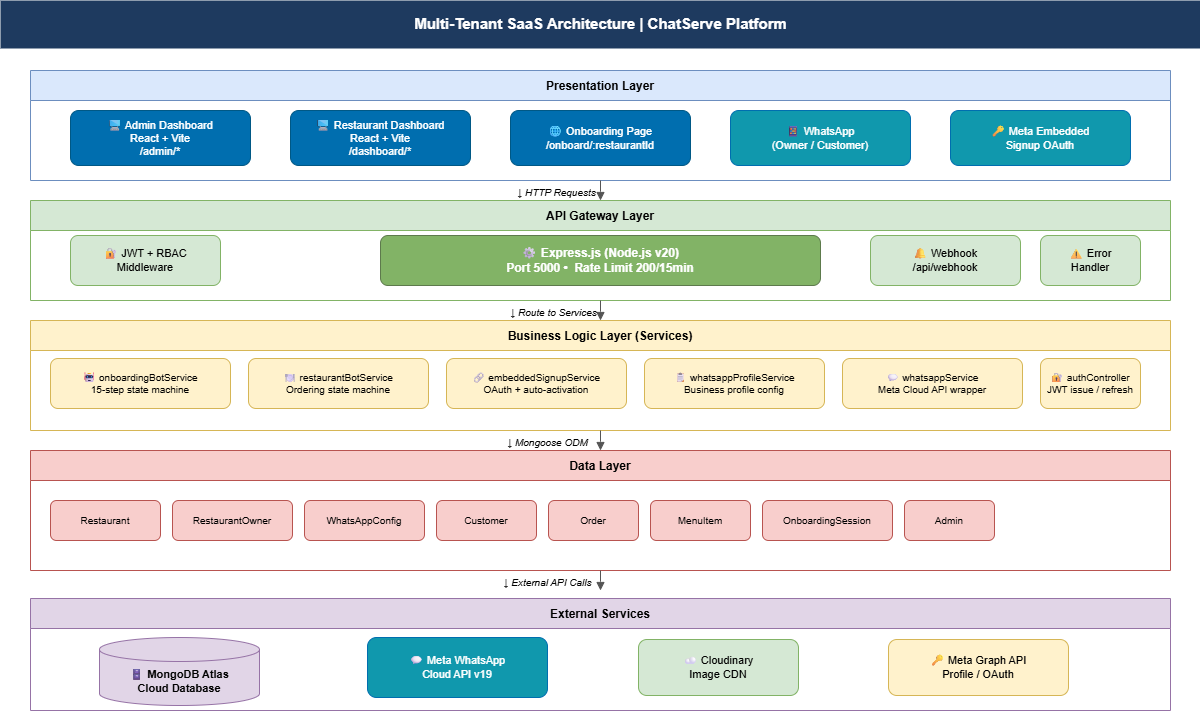
\includegraphics[width=0.78\textwidth]{system_architecture.png}
\end{center}

\small
\textbf{Layers:} React SPAs $\rightarrow$ Express.js API Gateway $\rightarrow$ Business Logic Services $\rightarrow$ MongoDB + Cloudinary + Meta WhatsApp API

\end{frame}

%==========================================================
% SLIDE: Onboarding Flow
%==========================================================
\section{System Flows}
\begin{frame}{Business Onboarding Flow}

\begin{center}
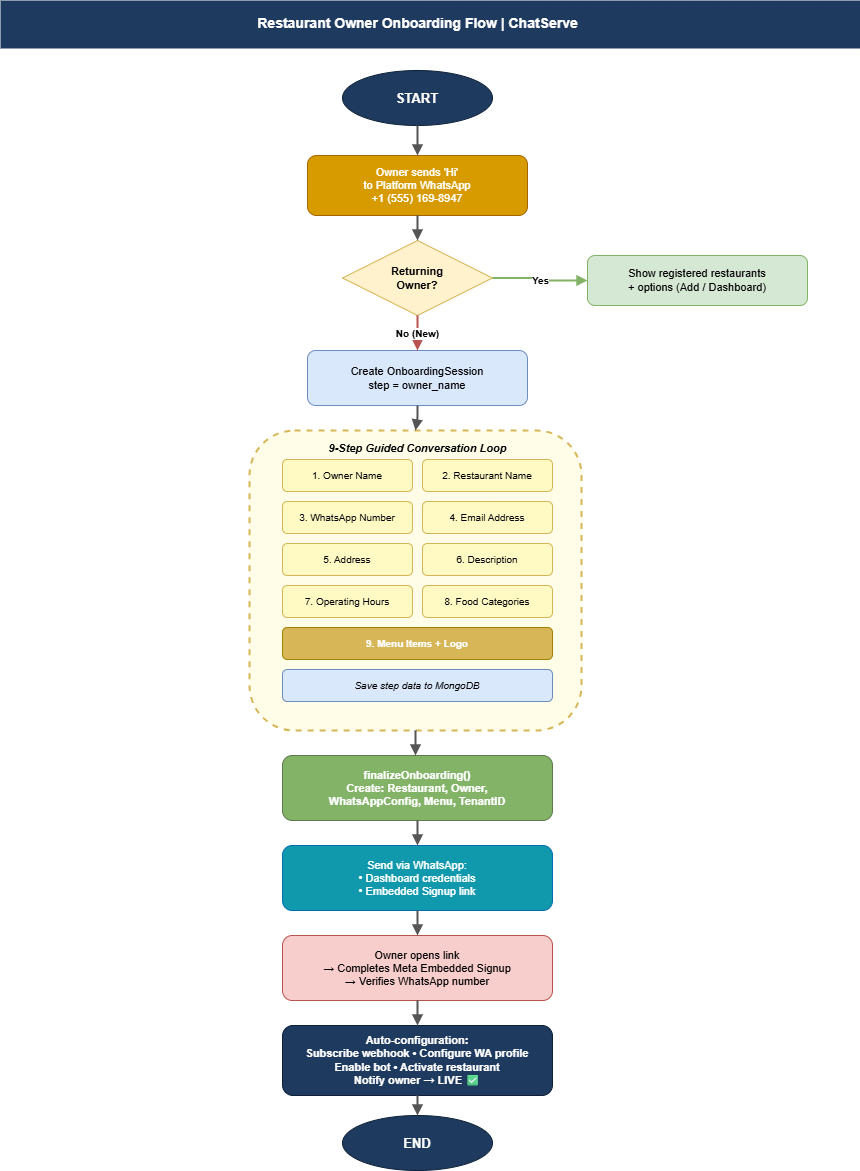
\includegraphics[width=0.72\textwidth]{Onboarding Flow.png}
\end{center}

\small
Owner sends ``Hi'' $\rightarrow$ Bot collects 10 details step-by-step $\rightarrow$ Account created $\rightarrow$ Embedded Signup link sent $\rightarrow$ WA API configured automatically

\end{frame}

%==========================================================
% SLIDE: Onboarding Sequence Diagram
%==========================================================
\begin{frame}{Onboarding -- Sequence Diagram}

\begin{center}
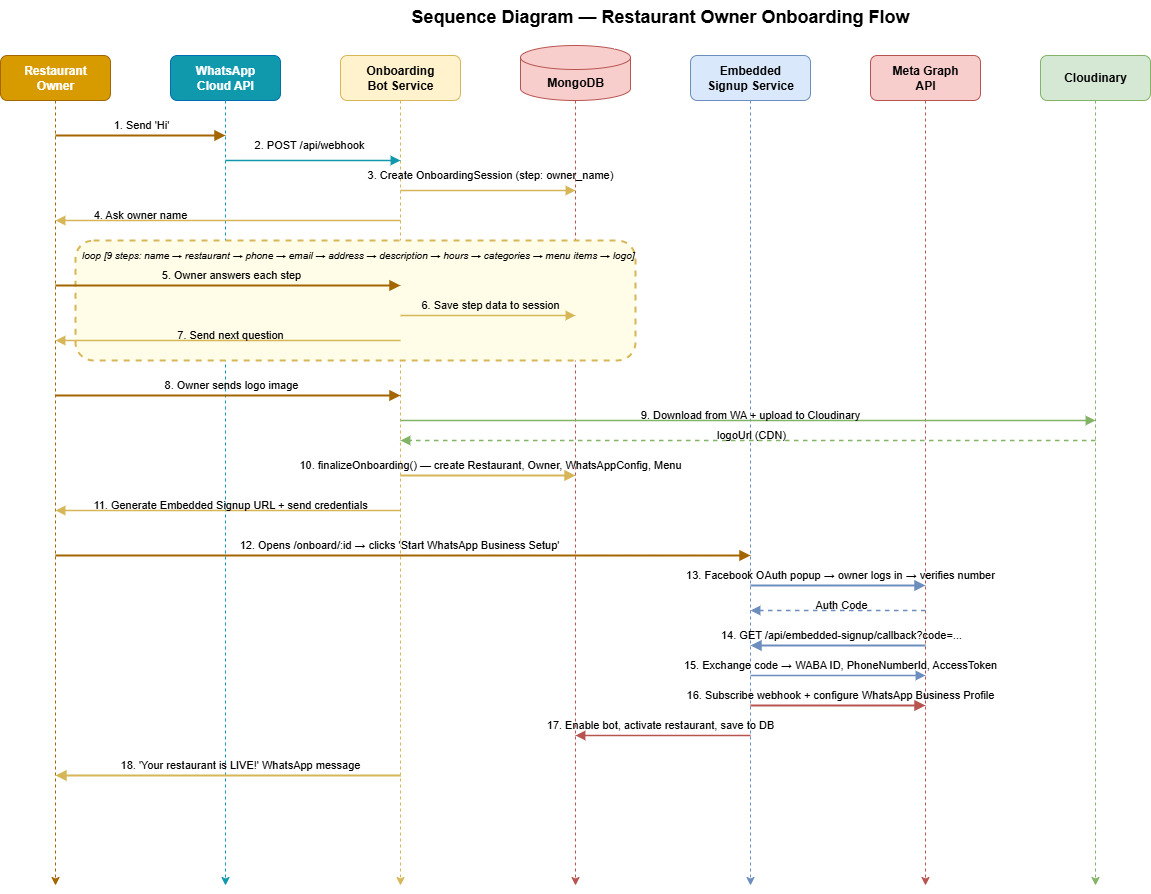
\includegraphics[width=0.82\textwidth]{Sequence_diagram - restauretn_Onboarding.png}
\end{center}

\end{frame}

%==========================================================
% SLIDE: Customer Order Flow
%==========================================================
\begin{frame}{Customer Order Flow}

\begin{columns}[T]
\begin{column}{0.48\textwidth}
\textbf{Order Processing Steps:}
\begin{enumerate}
  \item Customer messages business WA number
  \item Webhook routes to correct business bot
  \item Interactive main menu displayed
  \item Browse categories \& products/services
  \item Add items to persistent cart
  \item 3-step checkout (address $\rightarrow$ confirm $\rightarrow$ pay)
  \item Order confirmation with unique ID
  \item Status updates sent via WhatsApp
\end{enumerate}
\end{column}
\begin{column}{0.50\textwidth}
\begin{center}
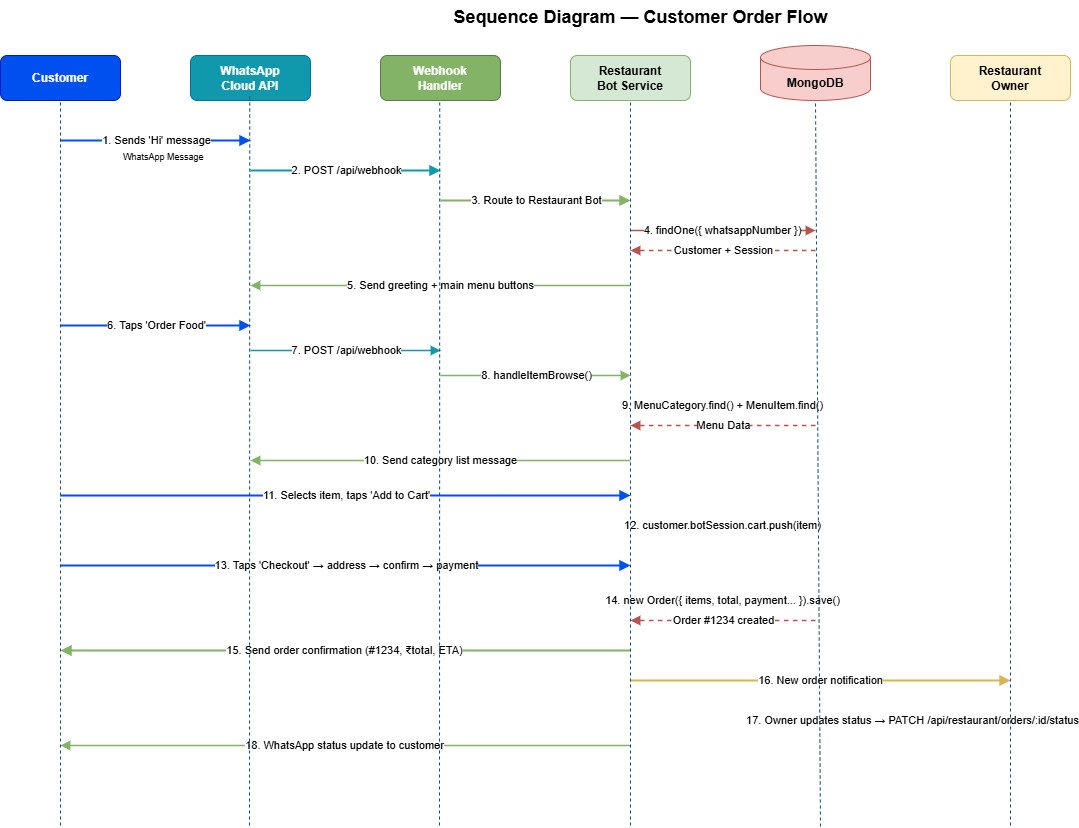
\includegraphics[width=\textwidth]{Sequence_Diagram- cutomer_Order Flow.png}
\end{center}
\end{column}
\end{columns}

\end{frame}

%==========================================================
% SLIDE: Database Design
%==========================================================
\section{Database Design}
\begin{frame}[shrink=5]{Database Design -- ER Diagram}

\begin{center}
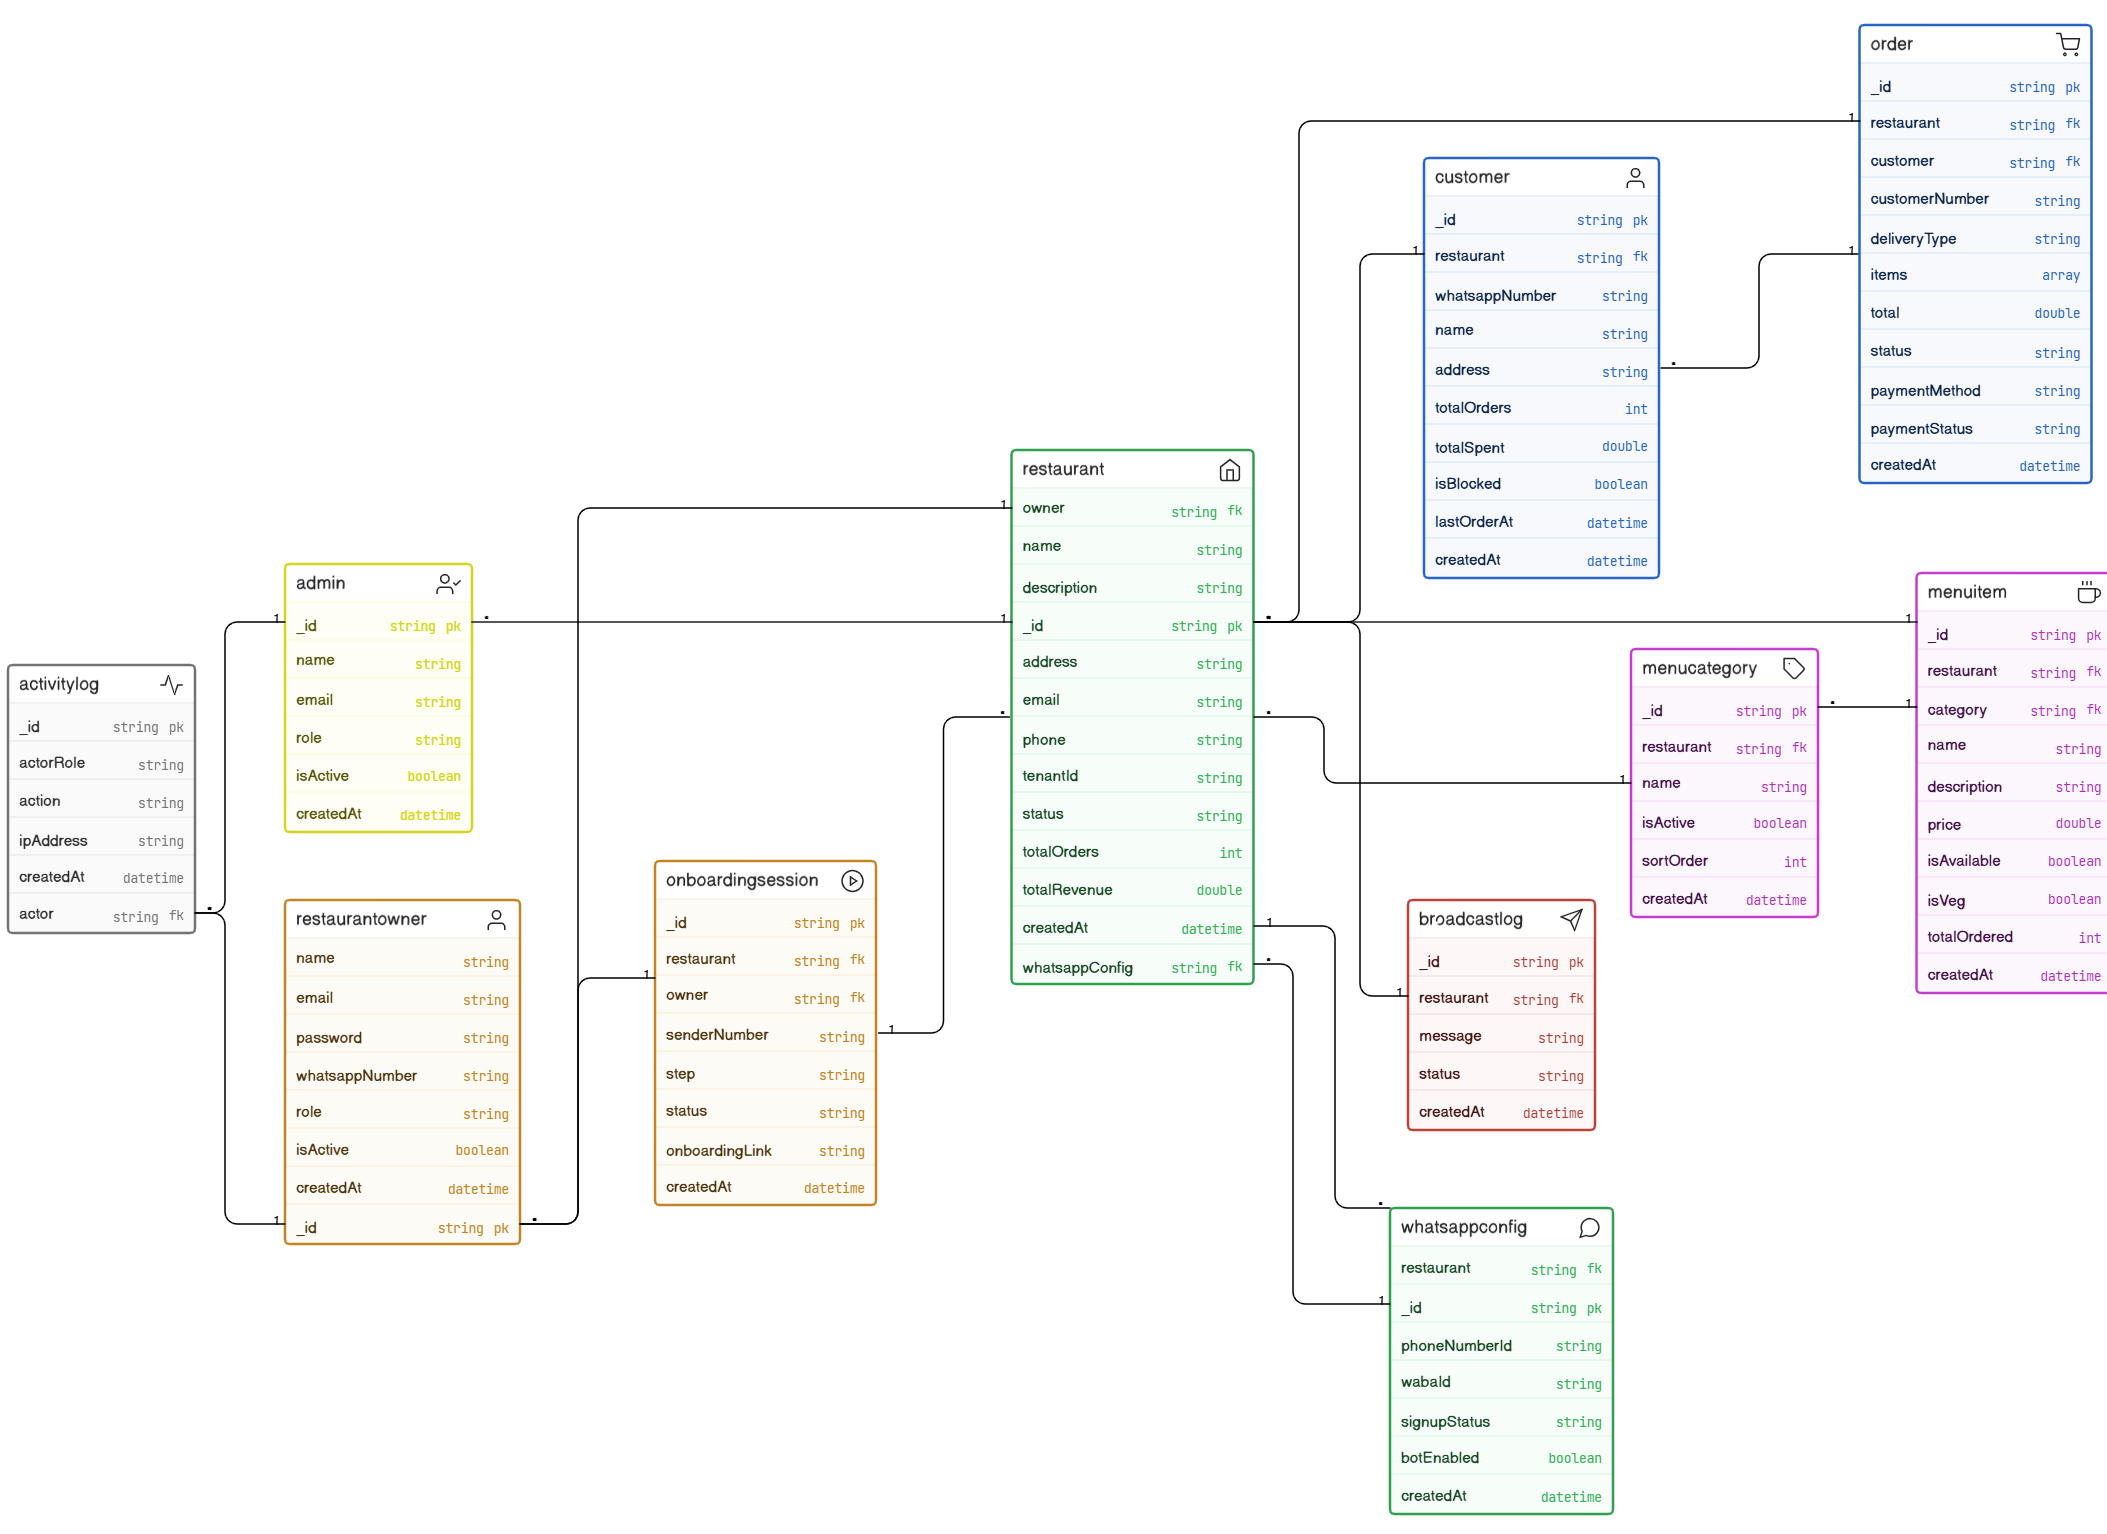
\includegraphics[width=0.70\textwidth]{er_diagram.png}
\end{center}

\small
\textbf{Multi-tenant MongoDB} -- Shared database, shared schema with \texttt{businessId} scoped queries for logical isolation.

\end{frame}

%==========================================================
% SLIDE: Database Collections
%==========================================================
\begin{frame}[shrink=5]{Core Database Collections}

\begin{columns}[T]
\begin{column}{0.48\textwidth}
\small
\begin{tabular}{ll}
\toprule
\textbf{Collection} & \textbf{Purpose} \\
\midrule
businesses & Core tenant document \\
businessowners & Auth \& contact info \\
whatsappconfigs & WABA credentials \\
customers & Session \& cart state \\
\bottomrule
\end{tabular}
\end{column}
\begin{column}{0.48\textwidth}
\small
\begin{tabular}{ll}
\toprule
\textbf{Collection} & \textbf{Purpose} \\
\midrule
catalogitems & Products/services \\
orders & Full order lifecycle \\
onboardingsessions & Registration progress \\
admins & Platform admin creds \\
\bottomrule
\end{tabular}
\end{column}
\end{columns}

\vspace{0.4cm}
\begin{block}{Multi-Tenancy Strategy}
Each record carries a \texttt{businessId} ObjectId. API queries are scoped to the authenticated tenant's ID at the middleware layer, ensuring full logical isolation while keeping infrastructure simple.
\end{block}

\end{frame}


%==========================================================
% SLIDE: Use Case Diagram
%==========================================================
\begin{frame}{Use Case Diagram}

\begin{center}
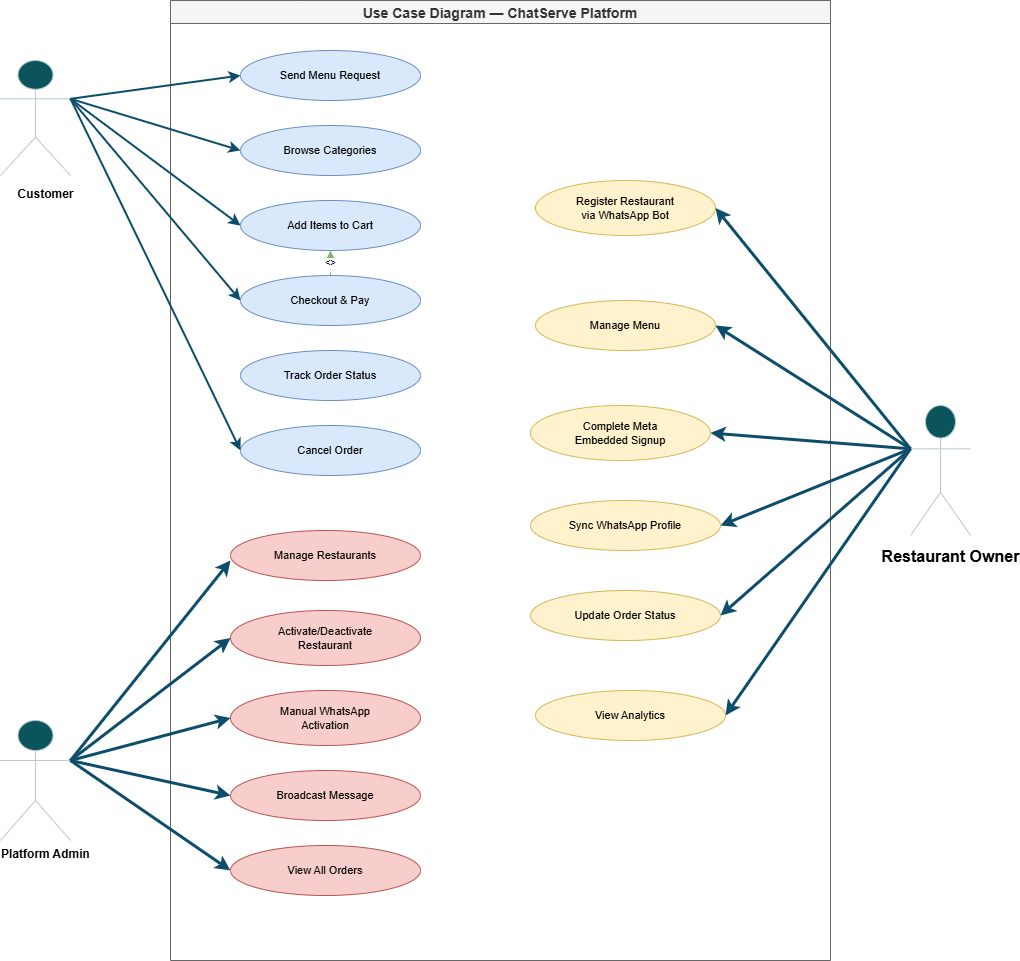
\includegraphics[width=0.72\textwidth]{Use Case Diagram.png}
\end{center}

\end{frame}

%==========================================================
% SECTION: Technology Stack
%==========================================================
\section{Technology Stack}
\begin{frame}{Technology Stack}

\begin{columns}[T]
\begin{column}{0.48\textwidth}
\textbf{Backend:}
\begin{itemize}
  \item Node.js 20.20 + Express.js 4.19
  \item MongoDB 7.x + Mongoose 8.4
  \item JWT (jsonwebtoken 9.0) + bcryptjs
  \item Cloudinary SDK for media
  \item Winston for logging
\end{itemize}
\vspace{0.3cm}
\textbf{External APIs:}
\begin{itemize}
  \item Meta WhatsApp Cloud API
  \item Meta Graph API
  \item Meta Embedded Signup OAuth
\end{itemize}
\end{column}
\begin{column}{0.48\textwidth}
\textbf{Frontend:}
\begin{itemize}
  \item React 18.3 + Vite 5.4
  \item Tailwind CSS 3.4
  \item TanStack Query 5.45
  \item Axios with interceptors
  \item Recharts for analytics
\end{itemize}
\vspace{0.3cm}
\textbf{Dev Tools:}
\begin{itemize}
  \item VS Code, Postman
  \item MongoDB Compass
  \item ngrok for webhook tunnelling
  \item Nodemon for hot reload
\end{itemize}
\end{column}
\end{columns}

\end{frame}

%==========================================================
% SECTION: Results / Demo Screenshots
%==========================================================
\section{Results}
\begin{frame}{Results -- WhatsApp Onboarding}

\begin{columns}
\begin{column}{0.48\textwidth}
\begin{center}
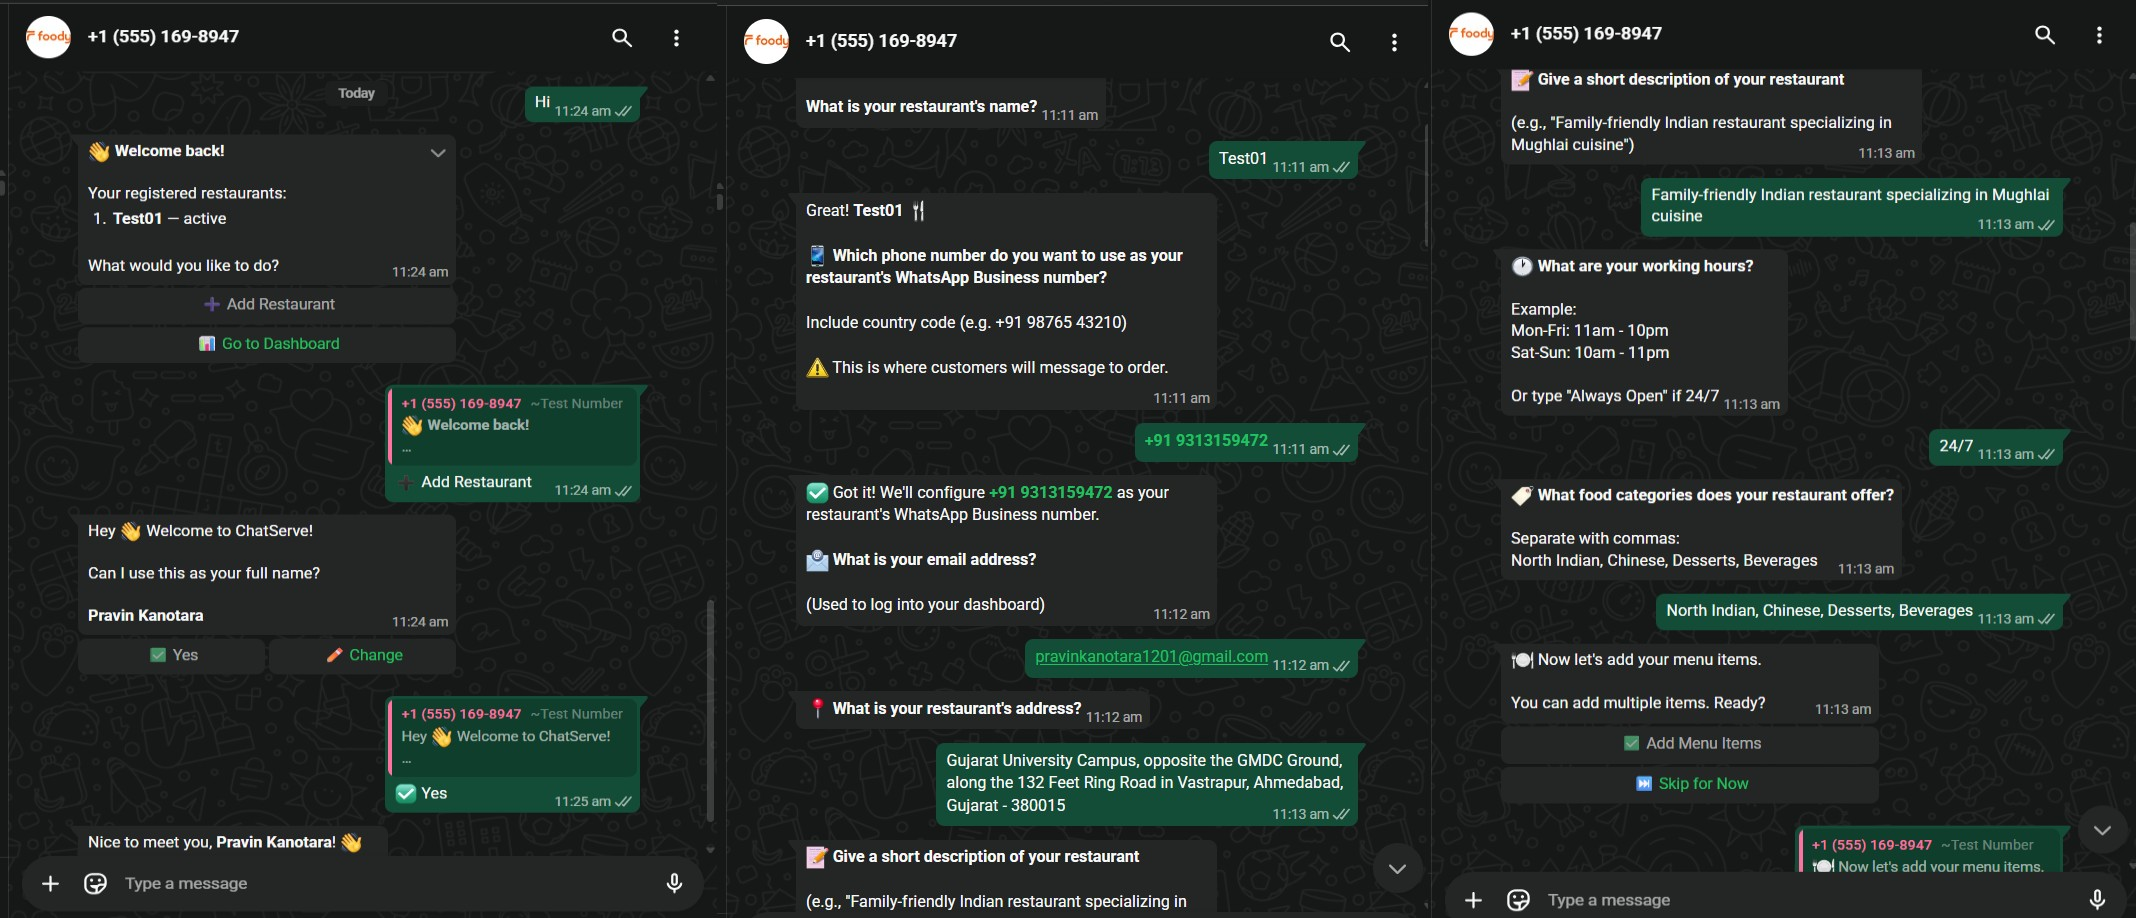
\includegraphics[width=0.85\textwidth]{restaurant_reg1_3.jpg}\\
\small (a) Steps 1--3: Name, Business, Phone
\end{center}
\end{column}
\begin{column}{0.48\textwidth}
\begin{center}
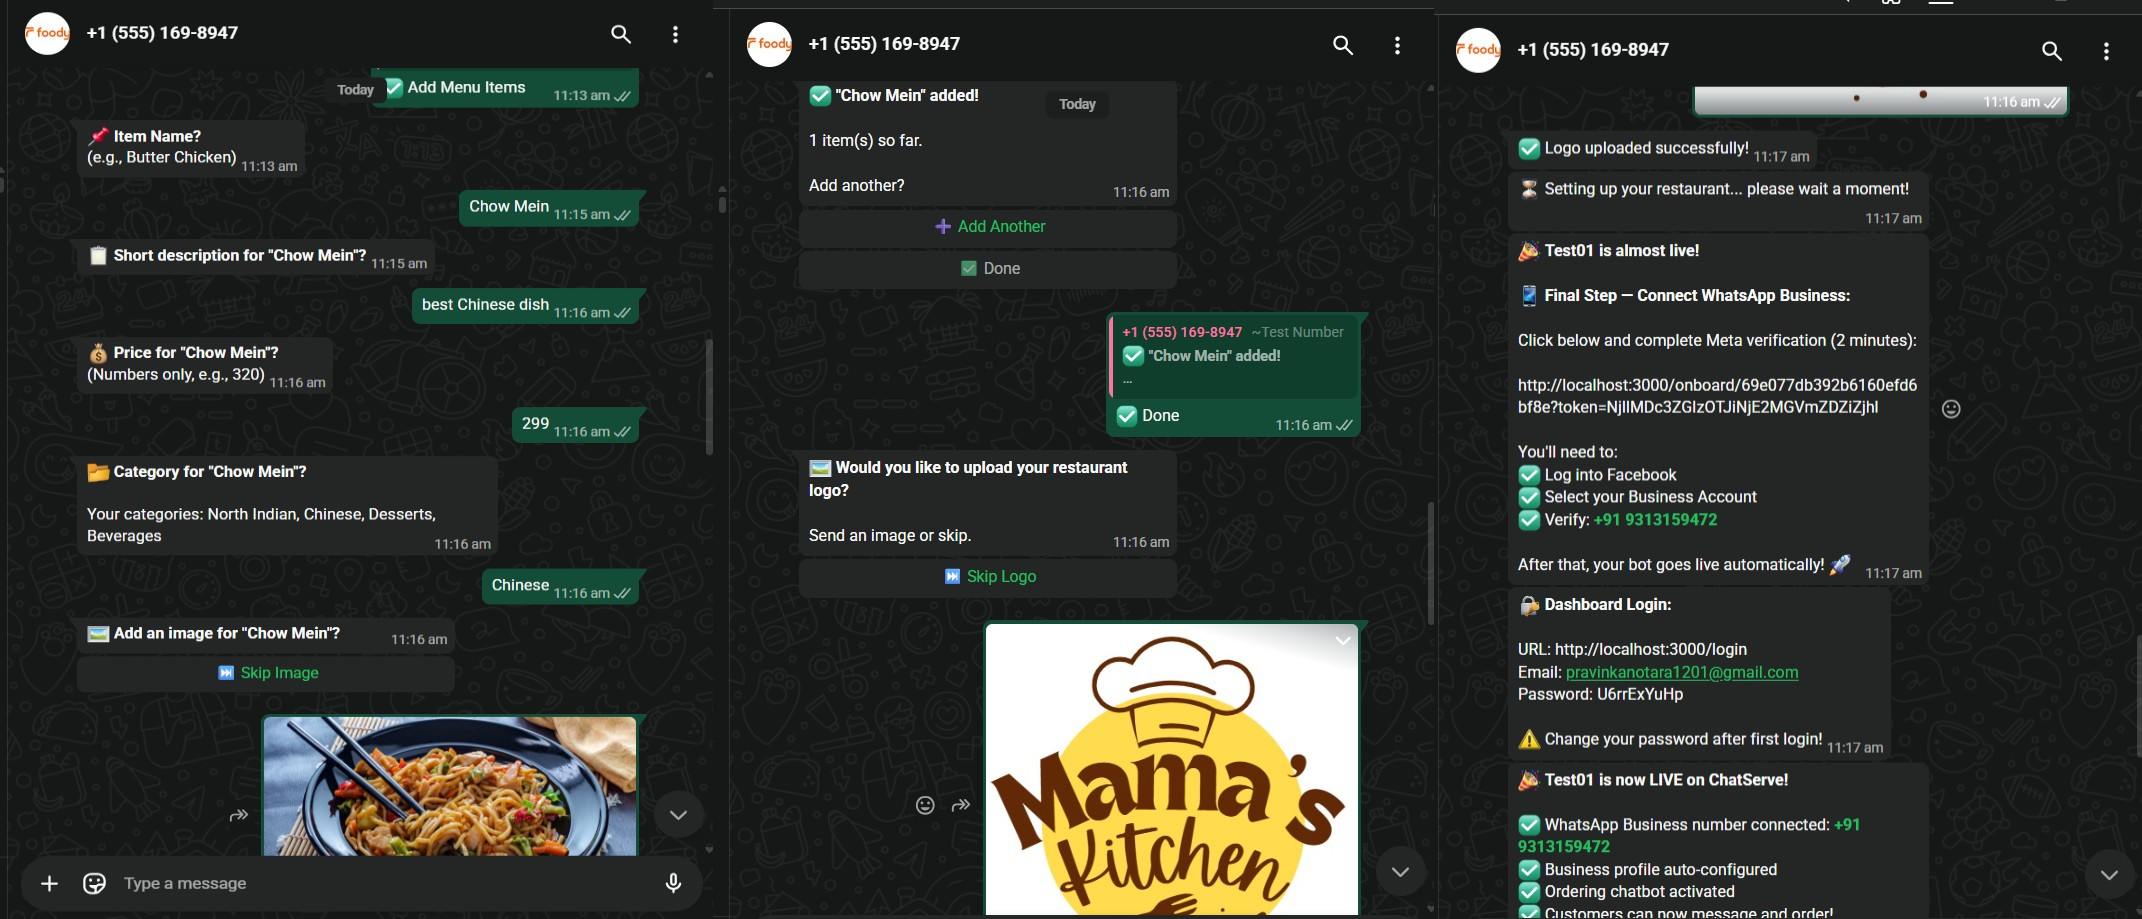
\includegraphics[width=0.85\textwidth]{restaurant_reg_4_6.jpg}\\
\small (b) Steps 4--6: Email, Address, Description
\end{center}
\end{column}
\end{columns}

\vspace{0.2cm}
\centering\small
Fully conversational onboarding -- no forms, no technical knowledge needed.

\end{frame}

%==========================================================
\begin{frame}[shrink=5]{Results -- Login \& Admin Dashboard}

\begin{columns}
\begin{column}{0.48\textwidth}
\begin{center}
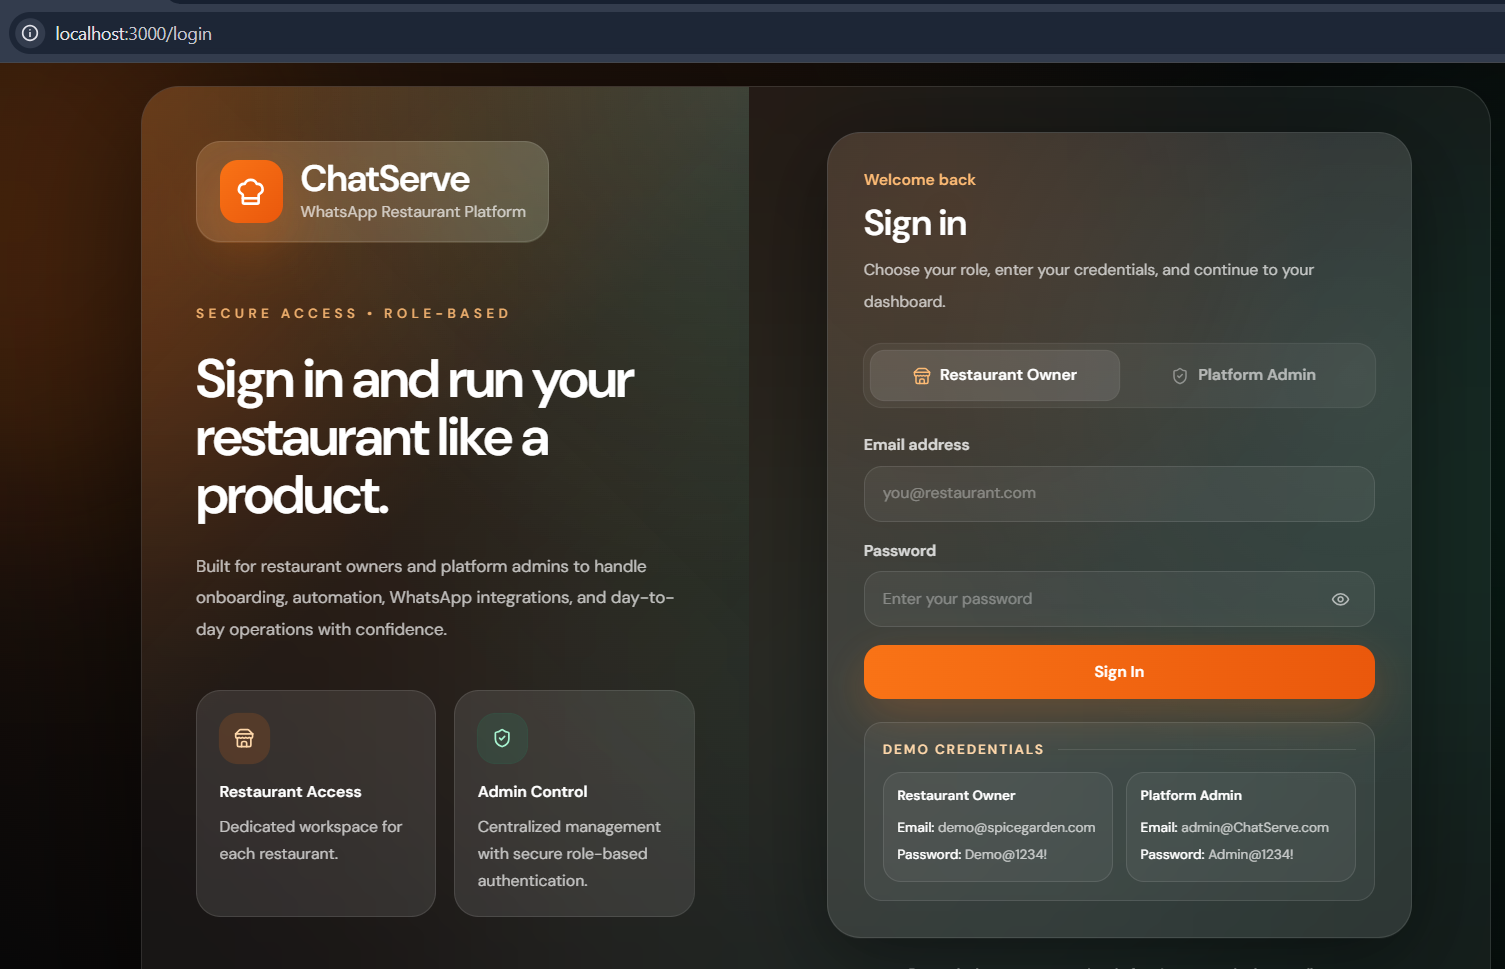
\includegraphics[width=\textwidth]{loginpage.png}\\
\small Role-based Login Page
\end{center}
\end{column}
\begin{column}{0.48\textwidth}
\begin{center}
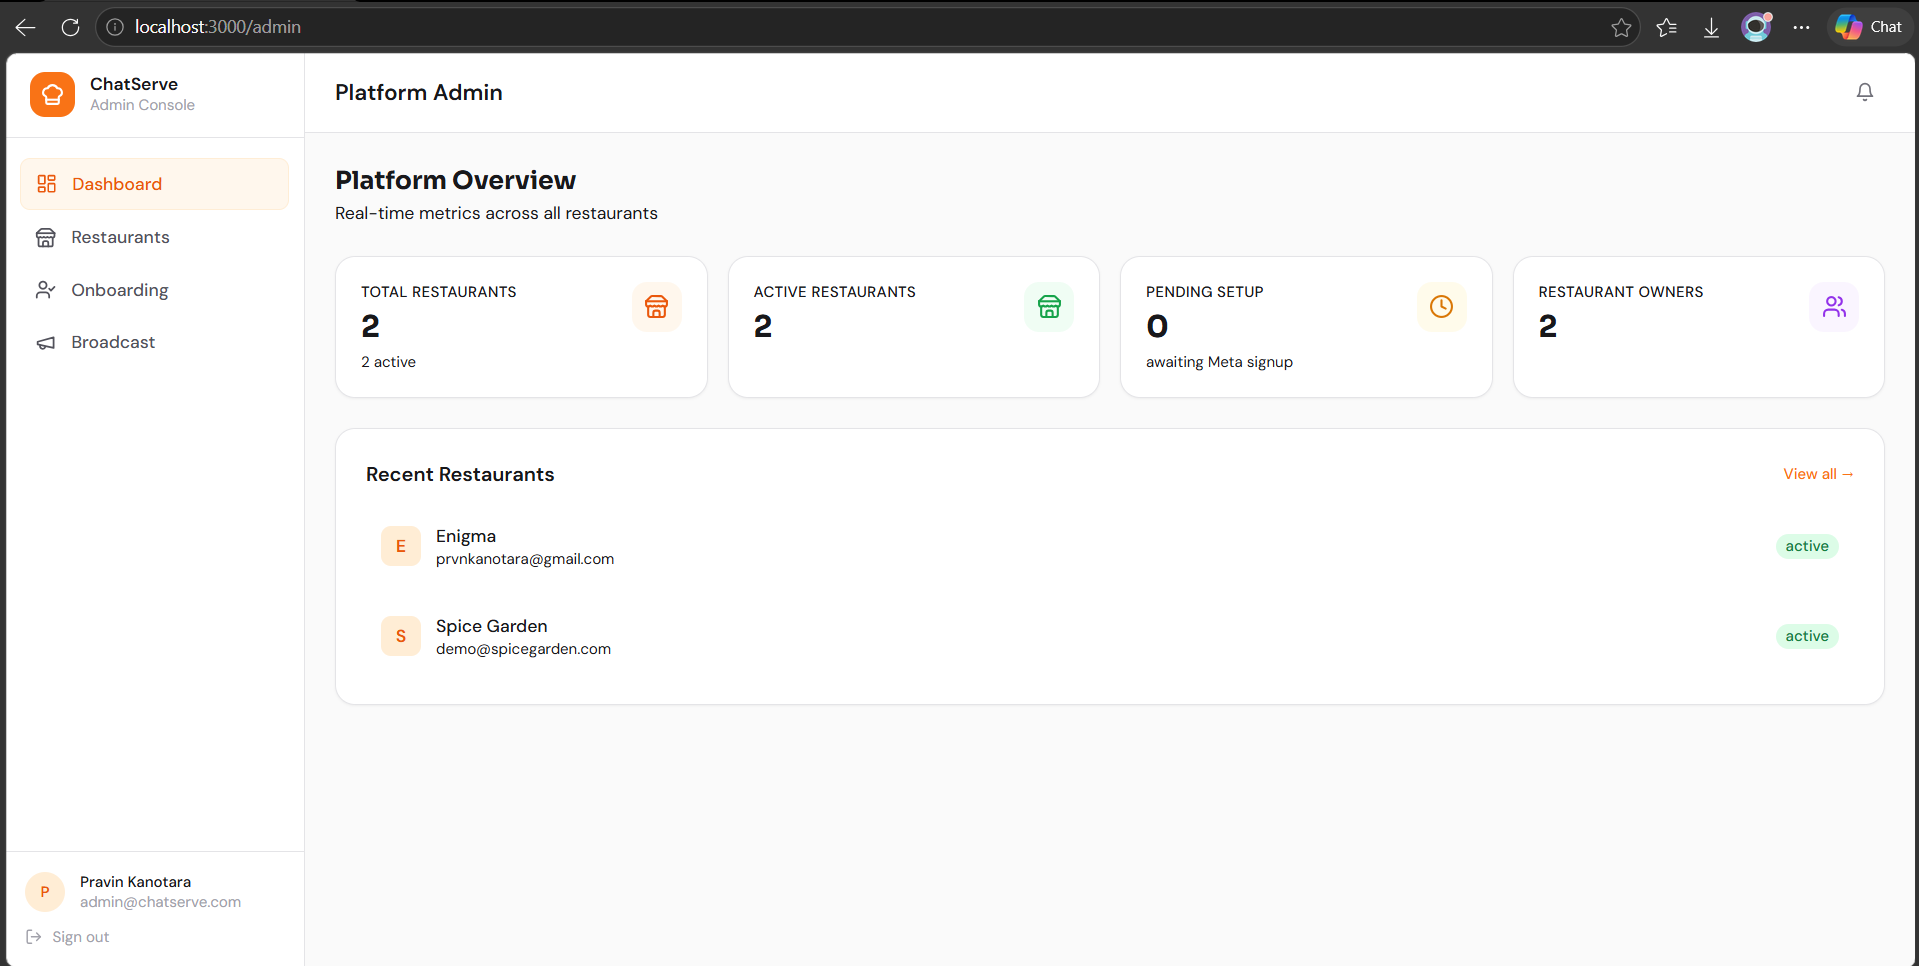
\includegraphics[width=\textwidth]{admin_dashboard .png}\\
\small Admin Dashboard -- Platform KPIs
\end{center}
\end{column}
\end{columns}

\end{frame}

%==========================================================
\begin{frame}[shrink=10]{Results -- Admin Controls}

\begin{columns}
\begin{column}{0.48\textwidth}
\begin{center}
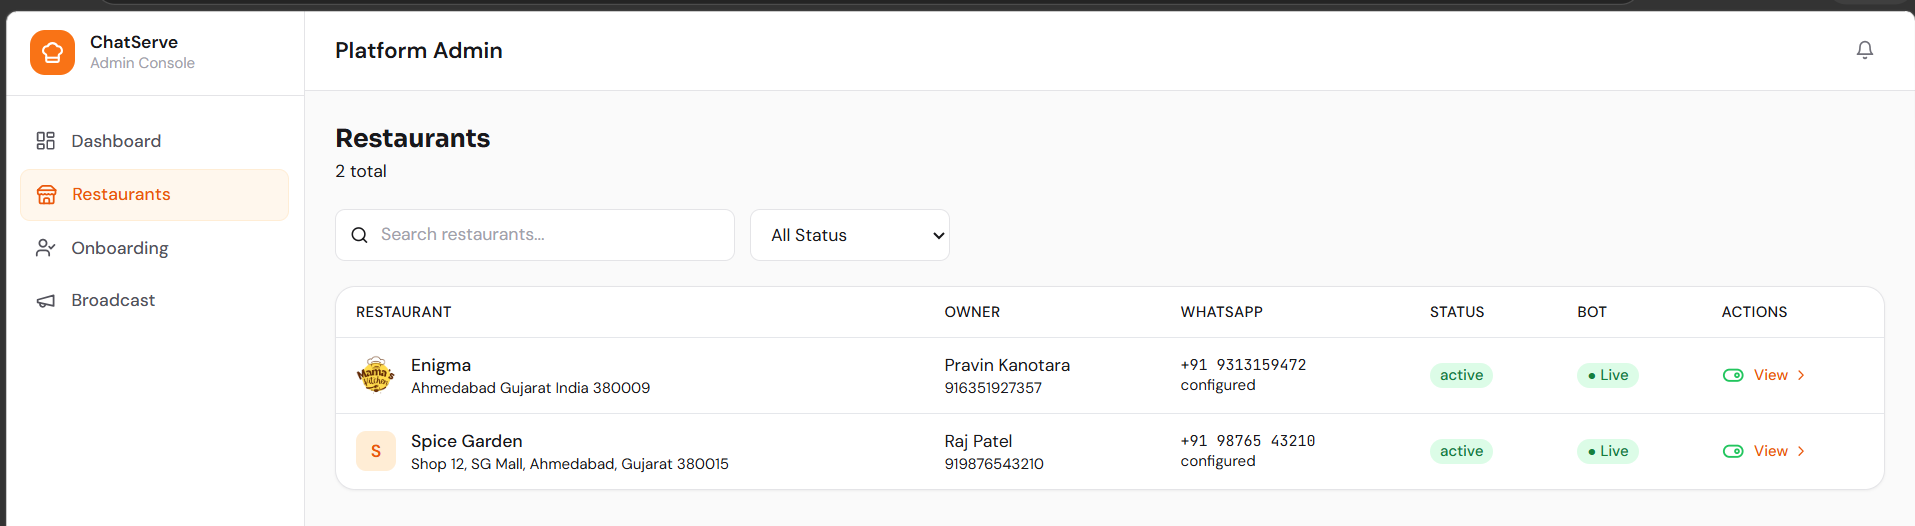
\includegraphics[width=\textwidth]{admin_restaurents.png}\\
\small Registered Businesses Listing
\end{center}
\end{column}
\begin{column}{0.48\textwidth}
\begin{center}
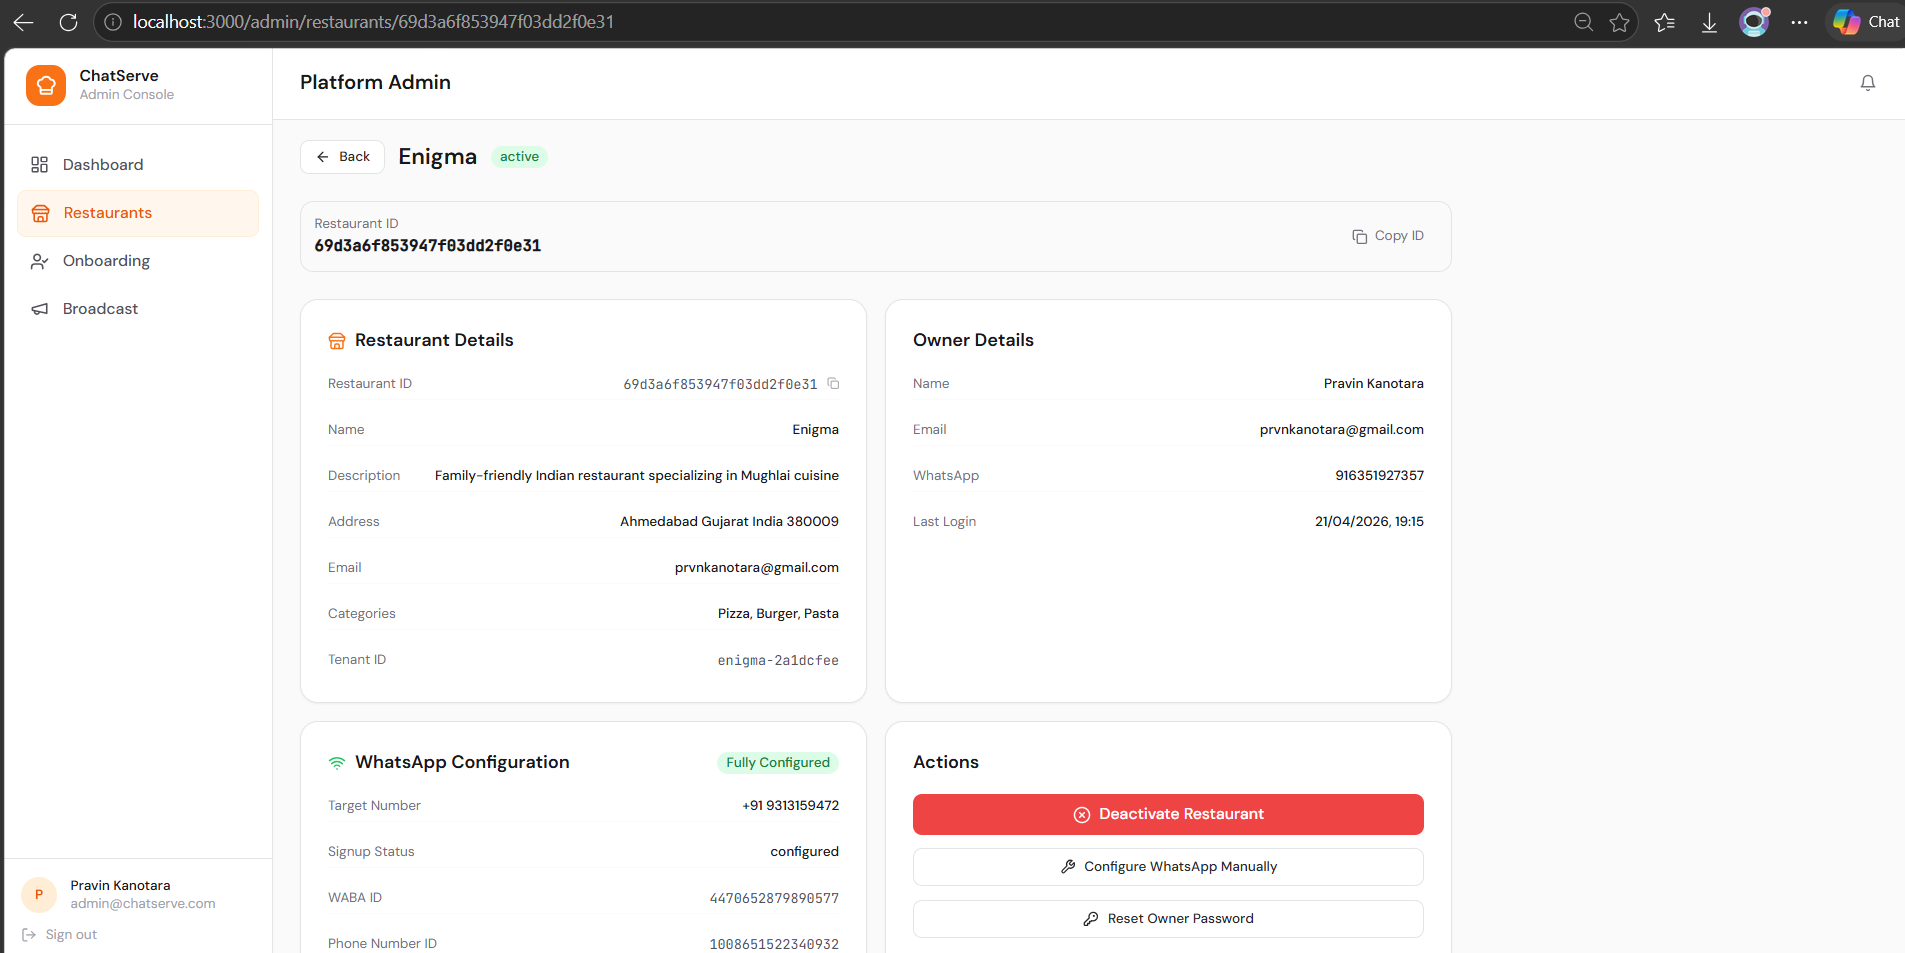
\includegraphics[width=\textwidth]{admin_restaurent_details.png}\\
\small Business Detail \& WA Config
\end{center}
\end{column}
\end{columns}

\vspace{0.2cm}
\begin{columns}
\begin{column}{0.48\textwidth}
\begin{center}
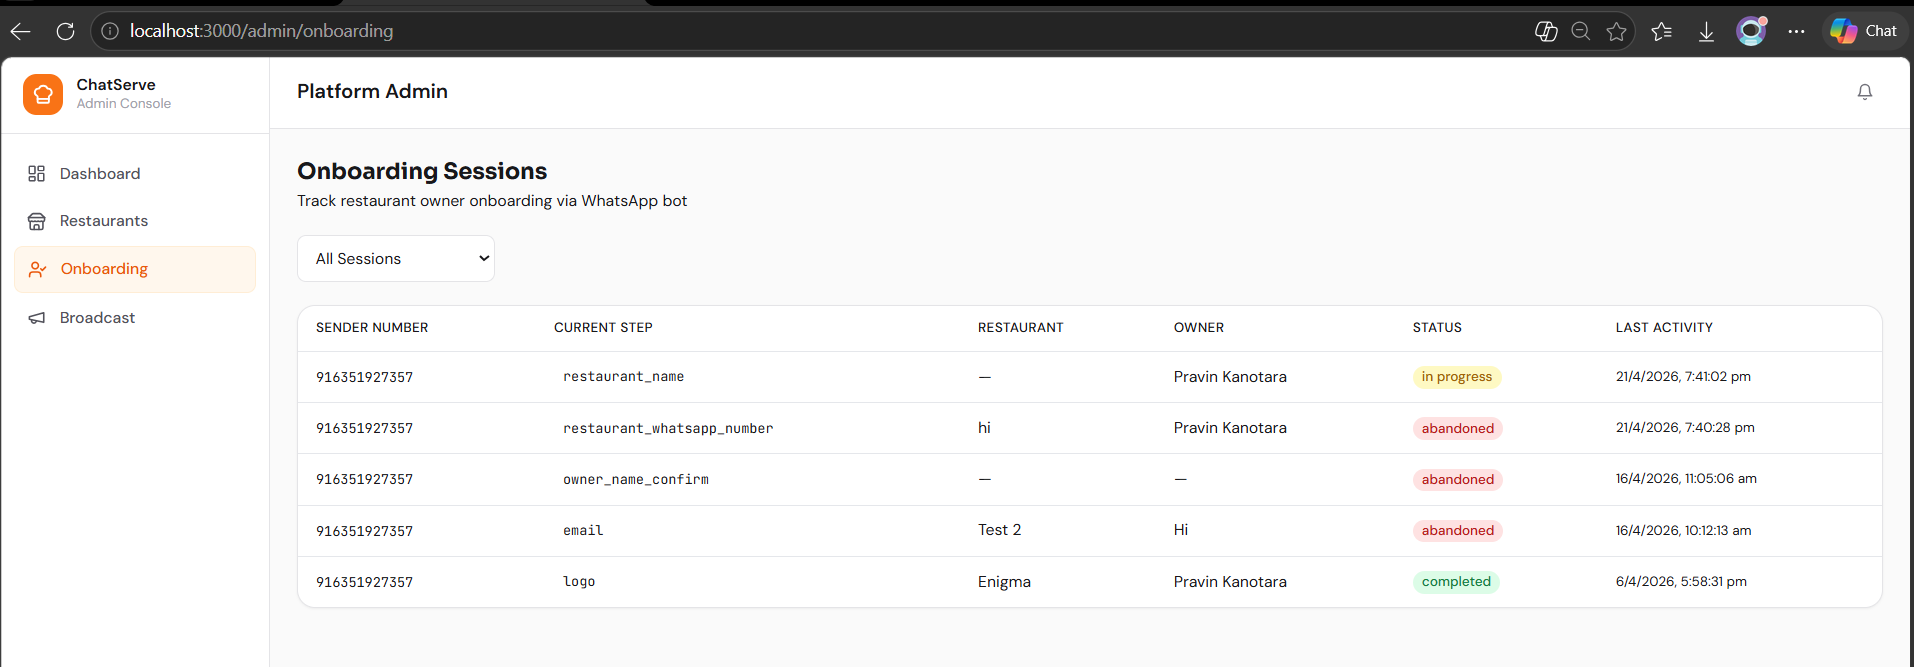
\includegraphics[width=\textwidth]{admin_onboarding.png}\\
\small Live Onboarding Monitor
\end{center}
\end{column}
\begin{column}{0.48\textwidth}
\begin{center}
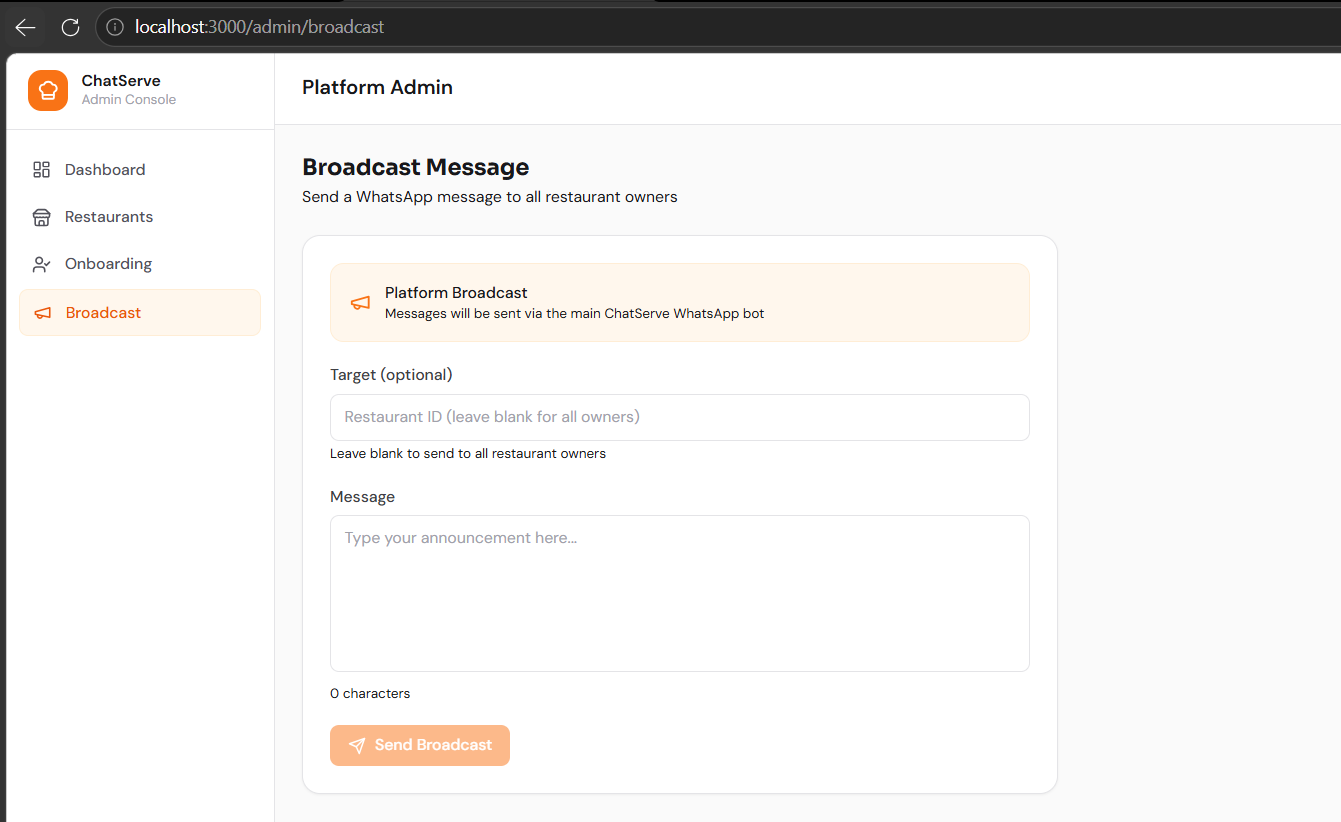
\includegraphics[width=\textwidth]{admin_brodcast.png}\\
\small Broadcast Messaging Module
\end{center}
\end{column}
\end{columns}

\end{frame}

%==========================================================
\begin{frame}[shrink=10]{Results -- Business Owner Dashboard}

\begin{columns}
\begin{column}{0.48\textwidth}
\begin{center}
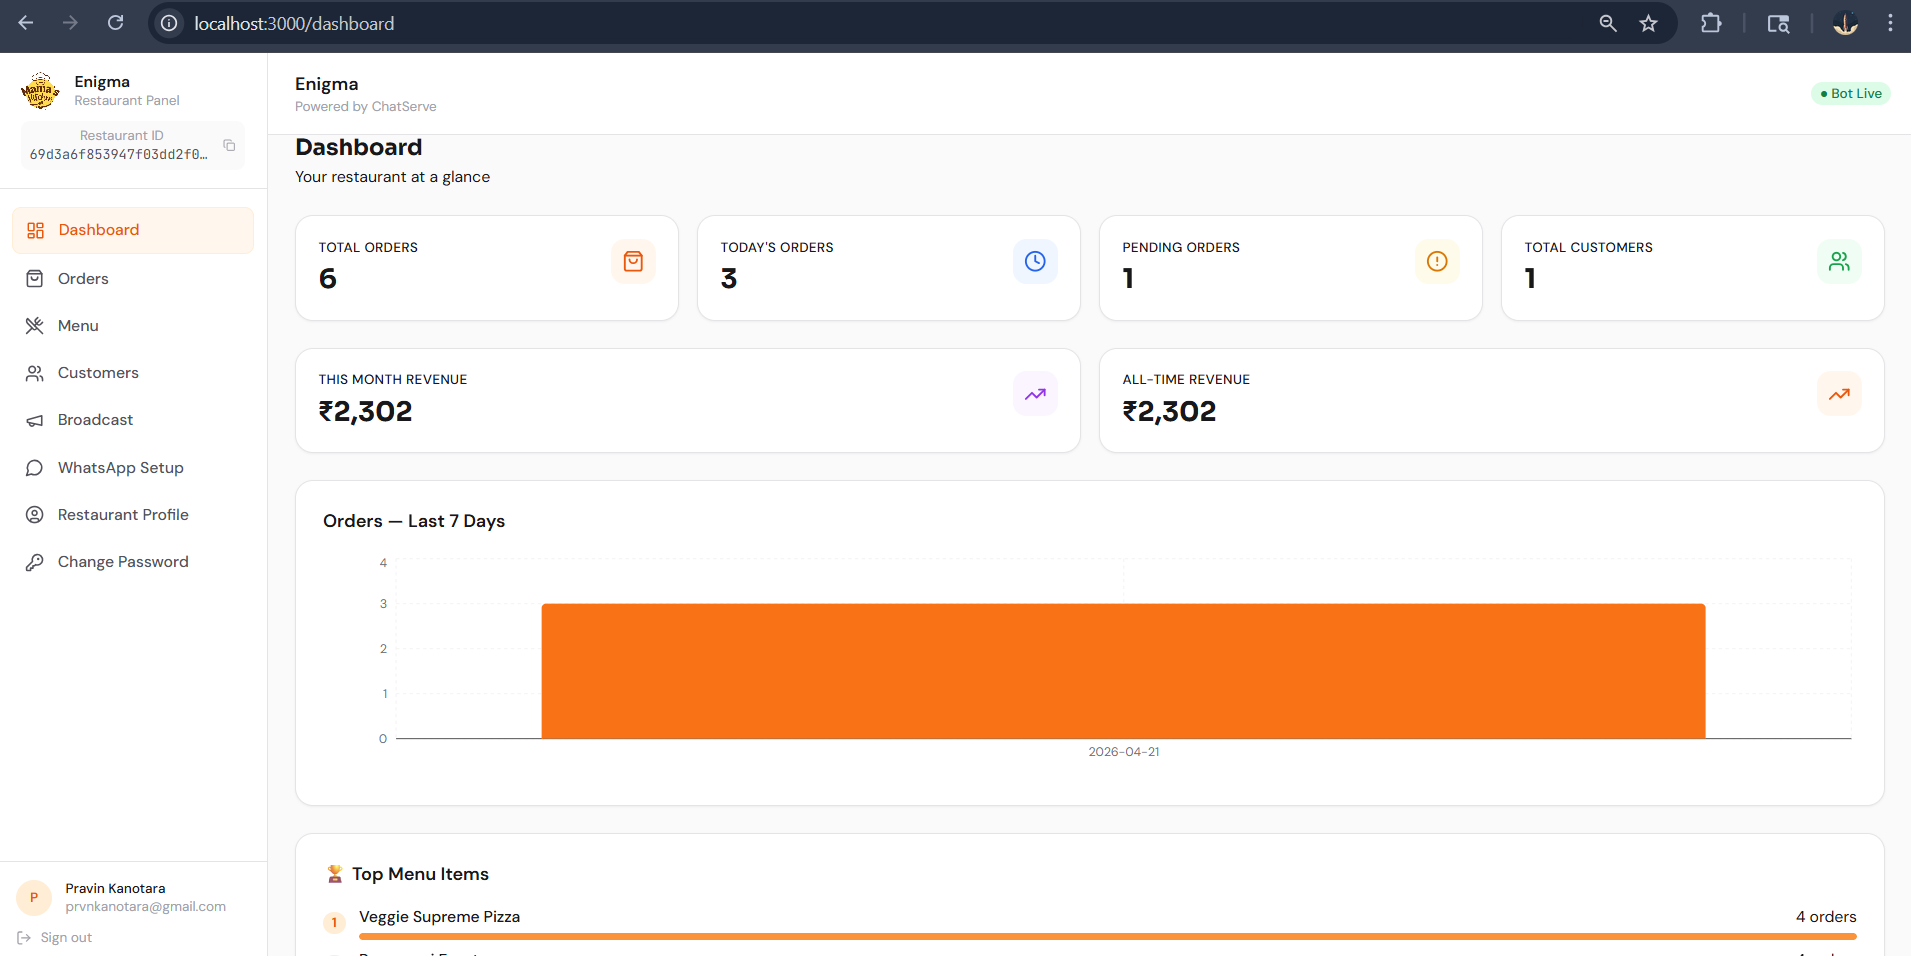
\includegraphics[width=\textwidth]{restaurant_dashboard.png}\\
\small Owner Dashboard -- Orders \& Revenue
\end{center}
\end{column}
\begin{column}{0.48\textwidth}
\begin{center}
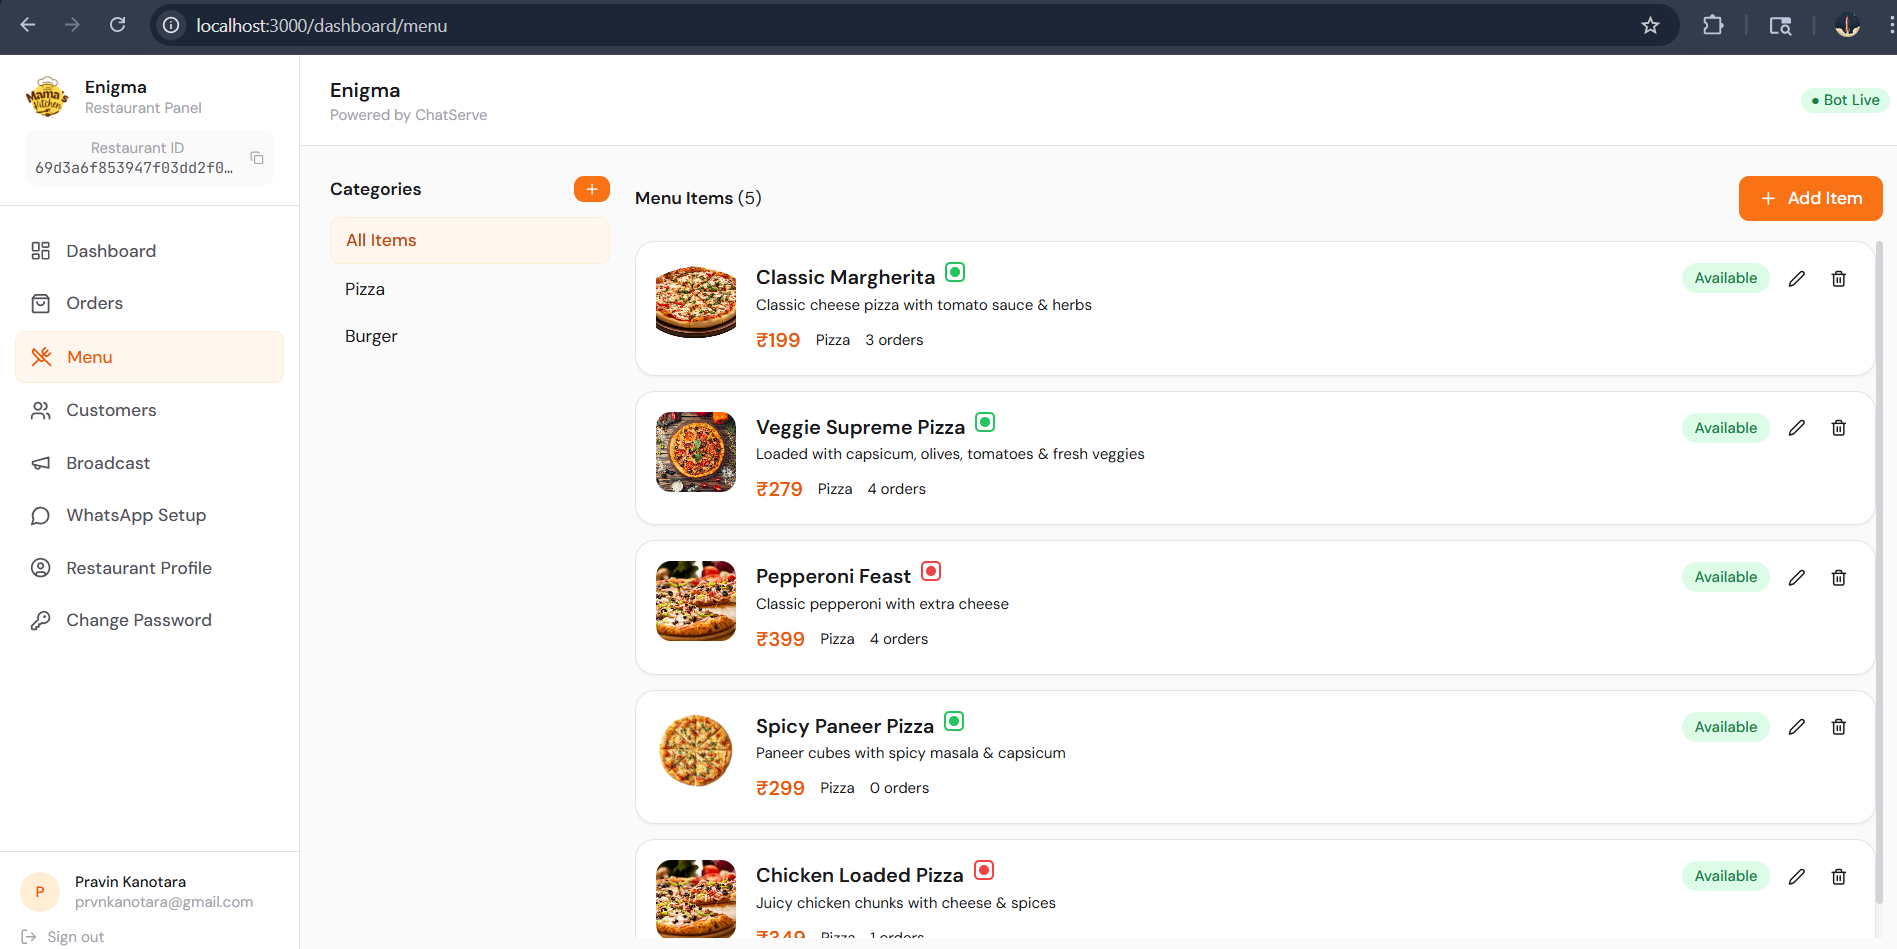
\includegraphics[width=\textwidth]{restaurant_menu.png}\\
\small Product/Service Catalog Management
\end{center}
\end{column}
\end{columns}

\vspace{0.2cm}
\begin{columns}
\begin{column}{0.48\textwidth}
\begin{center}
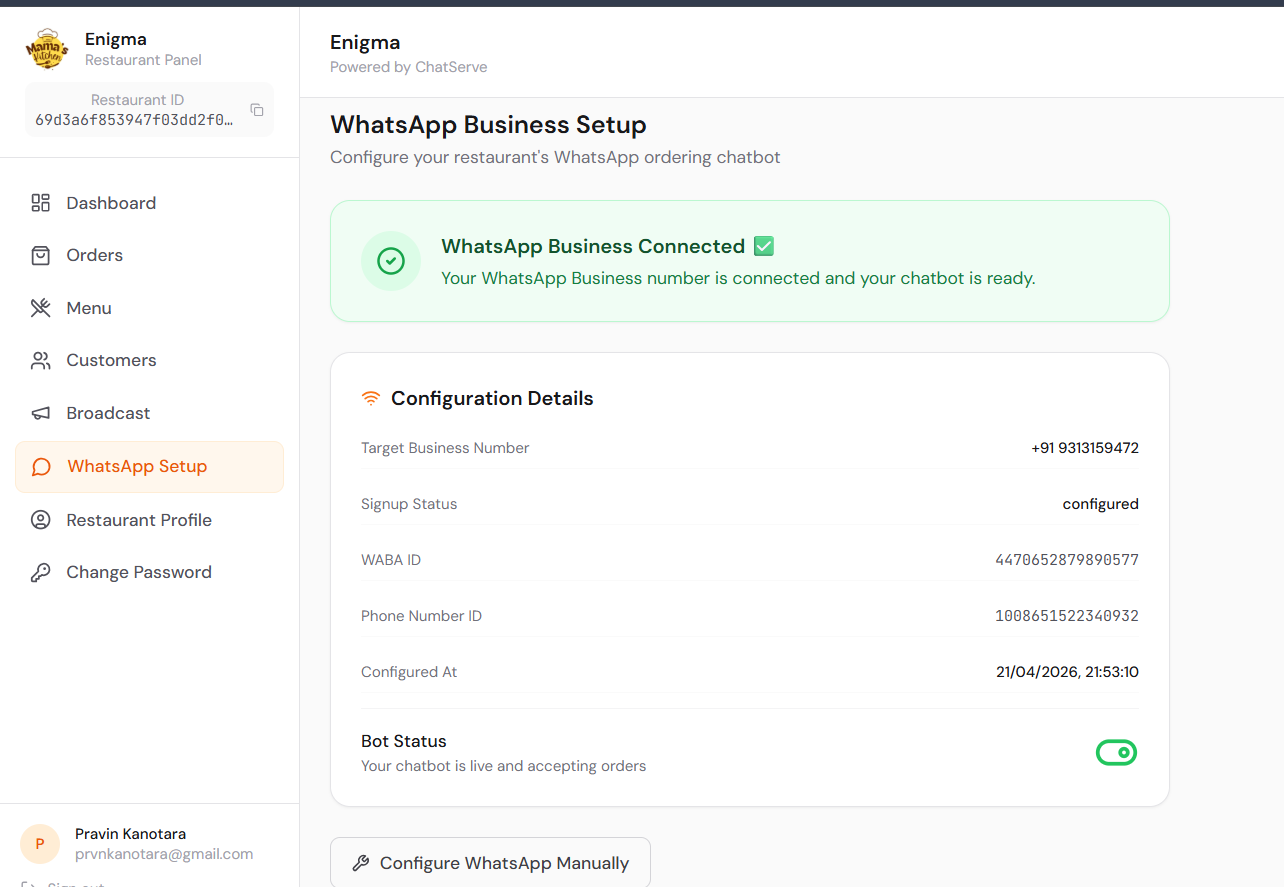
\includegraphics[width=\textwidth]{restaurant_WAprofile.png}\\
\small Auto-configured WA Business Profile
\end{center}
\end{column}
\begin{column}{0.48\textwidth}
\begin{center}
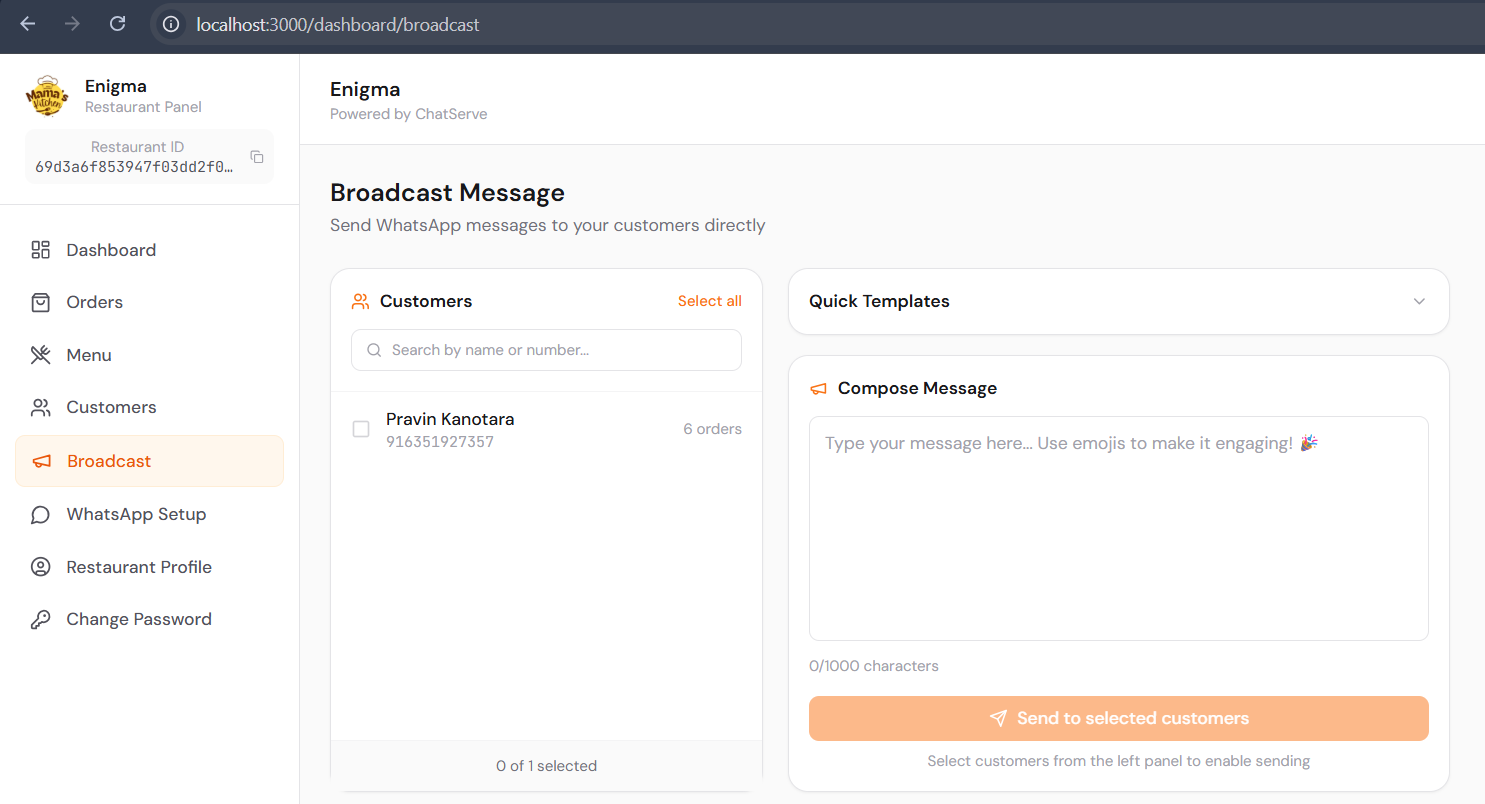
\includegraphics[width=\textwidth]{restaurant_brodcast.png}\\
\small Owner Broadcast Module
\end{center}
\end{column}
\end{columns}

\end{frame}

%==========================================================
% SECTION: Conclusion
%==========================================================
\section{Conclusion}
\begin{frame}[shrink=5]{Conclusion}

\begin{block}{Key Contributions}
\begin{itemize}
  \item Production-grade \textbf{multi-tenant WhatsApp SaaS} implementation
  \item Complete \textbf{Embedded Signup + OAuth} integration with auto post-configuration
  \item \textbf{State-machine driven dual-bot} architecture (onboarding + ordering)
  \item \textbf{Automatic WhatsApp Business Profile} sync from platform data
\end{itemize}
\end{block}

\vspace{0.2cm}
\begin{columns}[T]
\begin{column}{0.48\textwidth}
\textbf{Achievements:}
\begin{itemize}
  \item Reduces manual effort in order handling
  \item Improves customer response time
  \item Simplifies WhatsApp API integration
  \item Provides scalable, affordable solution
\end{itemize}
\end{column}
\begin{column}{0.48\textwidth}
\textbf{Limitations:}
\begin{itemize}
  \item Meta Business Verification needed for full production
  \item Free-tier cloud service constraints
  \item Dev access tokens require periodic renewal
\end{itemize}
\end{column}
\end{columns}

\end{frame}

%==========================================================
% SLIDE: Future Work
%==========================================================
\begin{frame}{Future Work}

\begin{columns}[T]
\begin{column}{0.32\textwidth}
\begin{block}{\small Near-Term (3--6 mo)}
\begin{itemize}\small
  \item Razorpay payment integration
  \item Full production deployment
  \item Template message system
\end{itemize}
\end{block}
\end{column}
\begin{column}{0.32\textwidth}
\begin{block}{\small Medium-Term (6--12 mo)}
\begin{itemize}\small
  \item Multi-language support (Hindi, Gujarati)
  \item Customer loyalty system
  \item NLP-based ordering
  \item Mobile app for owners
\end{itemize}
\end{block}
\end{column}
\begin{column}{0.32\textwidth}
\begin{block}{\small Long-Term (1+ year)}
\begin{itemize}\small
  \item Healthcare, tutoring, event verticals
  \item Multi-platform (Instagram, Telegram)
  \item Advanced analytics \& AI recommendations
\end{itemize}
\end{block}
\end{column}
\end{columns}

\end{frame}

%==========================================================
% SLIDE: References
%==========================================================
\begin{frame}{References}
\small
\begin{thebibliography}{9}
\bibitem{1} Meta Platforms Inc., ``WhatsApp Cloud API Documentation,'' \url{https://developers.facebook.com/docs/whatsapp/cloud-api}
\bibitem{2} Meta Platforms Inc., ``Embedded Signup for WhatsApp Business Platform,'' \url{https://developers.facebook.com/docs/whatsapp/embedded-signup}
\bibitem{3} PIB, ``MSME sector accounts for 30.1\% of India's GDP,'' Ministry of MSME, July 2025.
\bibitem{4} Infobip, ``WhatsApp statistics 2026: Market analysis \& global usage data,'' April 2026.
\bibitem{5} Hyperleap AI, ``WhatsApp Business Statistics India 2026,'' October 2025.
\bibitem{6} MSME Annual Report 2022--23, Ministry of MSME, Government of India.
\end{thebibliography}
\end{frame}

%==========================================================
% SLIDE: Thank You
%==========================================================
\section{}
\begin{frame}[plain]
\begin{center}
\vspace{1.5cm}
{\Huge\textbf{Thank You!}} \\
\vspace{0.5cm}
{\Large Questions?}\\
\vspace{0.8cm}
\normalsize
\textbf{Pravin Kanotara} (22BCE139)\\
\textit{Guide: Prof Monika Shah}\\
Department of Computer Science \& Engineering\\
Nirma University\\
\vspace{0.5cm}
\small
\texttt{pravin.kanotara@nirmauni.ac.in}
\end{center}
\end{frame}

\end{document}
